
% !TEX TS-program = pdflatex
% !TEX encoding = UTF-8 Unicode


%%%%%%%%%%%%%%%%%%%%%%%%%%%%%%%%%%%%%%%%%%%%%%%%%%%%%%%%%%%%%%%%%%%%%%
%%%%%%%%%%%%%%%%%%%%%%%%%%%%%%	HEADER %%%%%%%%%%%%%%%%%%%%%%%%%%%%%%%%%%%%
\documentclass[12pt]{article} 
\usepackage{amsmath, amsthm, amssymb} % AMS Math Package
\usepackage{graphicx} % Allows for eps images
\usepackage{multicol} % Allows for multiple columns
\usepackage{framed,color}
\usepackage{fancybox}
\usepackage{float}
\usepackage{caption,subcaption}
\usepackage{mathtools}
\usepackage{pgffor}
\usepackage{siunitx}

\usepackage{geometry}
\geometry{
top=0.5in,
inner=0.5in,
outer=0.5in,
bottom=0.5in,
headheight=1ex,
headsep=3ex
}


 % Sets margins and page size
\pagestyle{empty} % Removes page numbers
\makeatletter % Need for anything that contains an @ command 
\renewcommand{\maketitle} % Redefine maketitle to conserve space
{ \begingroup \vskip 10pt \begin{center} \large {\bf \@title}
	\vskip 10pt \large \@author \hskip 20pt \@date \end{center}
  \vskip 10pt \endgroup \setcounter{footnote}{0} }
\makeatother % End of region containing @ commands
\renewcommand{\labelenumi}{(\alph{enumi})} % Use letters for enumerate
% \DeclareMathOperator{\Sample}{Sample}
\let\vaccent=\v % rename builtin command \v{} to \vaccent{}
\renewcommand{\v}[1]{\ensuremath{\mathbf{#1}}} % for vectors
\newcommand{\gv}[1]{\ensuremath{\mbox{\boldmath$ #1 $}}} 
% for vectors of Greek letters
\newcommand{\uv}[1]{\ensuremath{\mathbf{\hat{#1}}}} % for unit vector
\newcommand{\abs}[1]{\left| #1 \right|} % for absolute value
\newcommand{\avg}[1]{\left< #1 \right>} % for average
\let\underdot=\d % rename builtin command \d{} to \underdot{}
\renewcommand{\d}[2]{\frac{d #1}{d #2}} % for derivatives
\newcommand{\dd}[2]{\frac{d^2 #1}{d #2^2}} % for double derivatives
\newcommand{\pd}[2]{\frac{\partial #1}{\partial #2}} 
% for partial derivatives
\newcommand{\pdd}[2]{\frac{\partial^2 #1}{\partial #2^2}} 
% for double partial derivatives
\newcommand{\pdc}[3]{\left( \frac{\partial #1}{\partial #2}
 \right)_{#3}} % for thermodynamic partial derivatives
\newcommand{\ket}[1]{\left| #1 \right>} % for Dirac bras
\newcommand{\bra}[1]{\left< #1 \right|} % for Dirac kets
\newcommand{\braket}[2]{\left< #1 \vphantom{#2} \right|
 \left. #2 \vphantom{#1} \right>} % for Dirac brackets
\newcommand{\matrixel}[3]{\left< #1 \vphantom{#2#3} \right|
 #2 \left| #3 \vphantom{#1#2} \right>} % for Dirac matrix elements
\newcommand{\grad}[1]{\gv{\nabla} #1} % for gradient
\let\divsymb=\div % rename builtin command \div to \divsymb
\renewcommand{\div}[1]{\gv{\nabla} \cdot #1} % for divergence
\newcommand{\curl}[1]{\gv{\nabla} \times #1} % for curl
\let\baraccent=\= % rename builtin command \= to \baraccent
\renewcommand{\=}[1]{\stackrel{#1}{=}} % for putting numbers above =
\newtheorem{prop}{Proposition}
\newtheorem{thm}{Theorem}[section]
\newtheorem{lem}[thm]{Lemma}
\theoremstyle{definition}
\newtheorem{dfn}{Definition}
\theoremstyle{remark}
\newtheorem*{rmk}{Remark}

\usepackage[utf8]{inputenc} % set input encoding (not needed with XeLaTeX)
\usepackage{tikz} %for making pretty figures
\usepackage[tikz]{bclogo}
\usepackage{tikz-3dplot}
\usetikzlibrary{calc}

%%% HEADERS & FOOTERS
\usepackage{fancyhdr}
\setlength{\headheight}{15pt}
\pagestyle{fancyplain}
\usepackage{lastpage}
\usepackage{siunitx}
\pagenumbering{arabic}

\lhead{Kyle Hoke}
\chead{PHYS 243A, Homework 1\rightmark}
\rhead{Page \thepage\ / \pageref{LastPage}}
\renewcommand{\headrulewidth}{0.4pt}
\fancyfoot[C]{}

%%% section* TITLE APPEARANCE
\usepackage{sectsty}
\allsectionsfont{\sffamily\mdseries\upshape} % (See the fntguide.pdf for font help)

%%% User Defined Commands %%%%
\newcommand{\f}[1]{f_{#1}(x)}
\newcommand{\axis}{
		\draw[->,thick](0,0) -- (0,5);
		\node[above] at (0,5) {$x$};
		\draw[->,thick](0,0) -- (5,0);
		\node[right] at(5,0){$y$};
		}

%%%%%%%%%%%%%%%%%%%%%%%%%%%%%%%%%%%%%%%%%%%%%%%%%%%%%%%%%%%%%%%%%%%%%%%%%%%%%%%
%%%%%%%%%%%%%%%%%%%%%%%%%%%%%%%%%%%%%% END OF HEADER %%%%%%%%%%%%%%%%%%%%%%%%%%%%%%%%%
%%%%%%%%%%%%%%%%%%%%%%%%%%%%%%%%%%%%%%%%%%%%%%%%%%%%%%%%%%%%%%%%%%%%%%%%%%%%%%%





%%% BEGIN DOCUMENT %%%%%%%%%%%%%%%%%%%%%%%%%%%%%%%%%%%%%%%%%%%%%%%%%%%%%%%%%%%%%%%%%%%
\title{\LARGE PHYS 243A Homework 1}
\author{Kyle Hoke}
%\date{} % Activate to display a given date or no date (if empty),
         % otherwise the current date is printed 

\begin{document}
\maketitle
\thispagestyle{empty}





%%%%%%%%%%%%%%%%%%%%%%%%%%%%%%%%%%%%%%%%%%%%%%%%%%%%%%%%%%%%%%%%%%%%%%%%%%%%%%%%%%%%
%%%%%%%%%%%%%%% PROBLEM 1 %%%%%%%%%%%%%%%%%%%%%
%%%%%%%%%%%%%%%%%%%%%%%%%%%%%%%%%%%%%%%%%%%%%%%%%%%%%%%%%%%%%%%%%%%%%%%%%%%%%%%%%%%%

\section*{1.1}

\begin{bclogo}[logo=\bcquestion , barre=none]
\newline
If we wish to produce a thin-film magnetic storage device with 100 Gbits/in$^2$, each bit is to be 5
times as big in one dimension as the other, the total amount of open area between bits is to be the
same as the total area occupied by the bits, and the film thickness of the medium storing the
information is to be 10 nm, how many atoms are involved in each bit? Assume for simplicity that the
film is pure Co, with a density of 9.0 x 1022 atoms/cm$^3$.
\end{bclogo}
\vspace{1cm}


Let's first visualize our bit with a nice image.

\begin{figure}[H]
 \centering
 \tdplotsetmaincoords{60}{125}
\begin{tikzpicture}
		[tdplot_main_coords,
			cube/.style={very thick,black},
			grid/.style={very thin,gray},
			axis/.style={->,blue,thick}]
	


	%draw the top and bottom of the cube
	\draw[cube] (0,0,0) -- (0,5,0) -- (2,5,0) -- (2,0,0) -- cycle;
	\draw[cube] (0,0,3) -- (0,5,3) -- (2,5,3) -- (2,0,3) -- cycle;
	
	%draw the edges of the cube
	\draw[cube] (0,0,0) -- (0,0,3);
	\draw[cube] (0,5,0) -- (0,5,3);
	\draw[cube] (2,0,0) -- (2,0,3);
	\draw[cube] (2,5,0) -- (2,5,3);
	
	%place labels on the cube edges
	\draw(2,0,1.5) node[anchor=east]{$x$};
	\draw(2,2.5,0) node[anchor=north]{$5x$};
	\draw(1, 5, 0) node[anchor=north west]{$10 nm$};
	
\end{tikzpicture}
 \caption{A single bit}
 \label{bit}
\end{figure}

We are told that we want 100 Gbits/in$^2$ and that half of the area is open, thus 
\[
	A_{bits} = 0.5 \,\, \text{in}^2  = 3.23 \times 10^{-4} \,\, \text{m}^2.
\]

Each square inch contains 100 Gbits or $10^11$ bits. We can compare this to the knowledge that a single  bit has an cross sectional area of $A = 5x^2$, so we set up a simple ratio to solve for $x$:

\begin{align*}
	\dfrac{3.23\times 10^{-4} \,\text{m}^2}{10^{11} \,\text{bits}} &= \dfrac{5x^2\,\text{m}^2}{1 \text{bit}}\\[3mm]
	x &= \sqrt{\dfrac{3.23\times10^{-4}}{5\times10^{11}}}\,\,\text{m} \\[3mm]
	x &= 2.54\times 10^{-8} \,\text{m}\\[3mm]
	x &= 25.4 \, \text{nm}
\end{align*}

We can now directly calculate the volume of the bit as pictured in Figure \ref{bit}.
\begin{align*}
	V_{bit\_stack} &= 5(25.4)^2 10\\[3mm]
		&=  32258\,\,\text{nm}^3\\[3mm]
		&= 3.23\times 10^{-17} \,\,\text{cm}^3
\end{align*}

Now we can use the density of Co atoms to find out how many atoms are in a single bit.
\[
\dfrac{3.23\times 10^{-17}\,\text{cm}^3}{1\,\text{bit}} \cdot \dfrac{9\times10^{22}\,\text{atoms}}{1\,\text{cm}^3} = \boxed{ \dfrac{2.9\times 10^6 \,\text{atoms}}{1\,\text{bit}} }
\]

%%%%%%%%%%%%%%%%%%%%%%%%%%%%%%%%%%%%%%%%%%%%%%%%%%%%%%%%%%%%%%%%%%%%%%%%%%%%%%%%%%%%
%%%%%%%%%%%%%%% PROBLEM 2 %%%%%%%%%%%%%%%%%%%%%
%%%%%%%%%%%%%%%%%%%%%%%%%%%%%%%%%%%%%%%%%%%%%%%%%%%%%%%%%%%%%%%%%%%%%%%%%%%%%%%%%%%%
\newpage
\section*{1.2}

\begin{bclogo}[logo=\bcquestion , barre=none]
\newline
(a) Begin with the Maxwell-Boltzmann distribution for molecular velocities in an ideal gas as
expressed in x,y,z coordinates, and derive by integration the formula for the rate at which molecules
strike a flat surface of unit area perpendicular to one of the axes. From this, determine the time
necessary to form a monolayer of gas on a surface, assuming a general sticking probability of PS. Note
that this is the same derivation that can be found in many physical chemistry texts to predict the rate at
which a gas leaks out through an orifice.
\newline
(b) Now make the assumption that only the bare surface area remaining on the surface after a given
exposure time is active for a particular gas adsorption, and that PS = unity on the bare area, but zero
elsewhere. Derive the general form of PS as a function of time for this case.\newline
(c) If a surface is exposed to 10$^{-9}$ Torr of CO at ambient temperature, how long will it take to form the first monolayer:
\newline 
(i) If Ps = unity?
\newline 
(ii) If Ps follows the relationship of part (b)?
\end{bclogo}
\vspace{2cm}

\subsection*{Part a:}
We begin with the Maxwell-Boltzmann distribution for molecules in an ideal gas.
\[
D(v) = \sqrt{\left(\dfrac{m}{2\pi kt}\right)^3}4\pi v^2 \exp{\left(-\dfrac{mv^2}{2kt}\right)}
\]

Where $D$ is the probability of finding a molecule at speed $v$. The speed $v^2 = v_x^2 + v_y^2 + v_z^2$ is in three dimensions. We first want to find the average speed of the molecules, then the flux through a single side of a unit cube when the molecules have a given number density. To find an average speed we add all the speeds up weight by their probability.
\[
	\bar{v}  = \sum v D(v) \Delta v,
\]
where $\Delta v$ represents a discrete spacing of speeds. In reality we can have continuum of speeds so to find the average speed we must sum over all possible speeds, which means an integral.

\begin{align*}
	\bar{v} &= \int_{0}^{\infty} v D(v) dv \\[3mm]
		&= \int_{0}^{\infty} \sqrt{\left(\dfrac{m}{2\pi kt}\right)^3}4\pi v^3 \exp{\left(-\dfrac{mv^2}{2kt}\right)} \\[3mm]
		&= \left(\dfrac{m}{2\pi kt}\right)^{3/2} 4\pi \int_{0}^{\infty} v^3 \exp{\left(-\dfrac{mv^2}{2kt}\right)}
\end{align*}
	
Now we make a substitution to make the integration easier: $$x = mv^2/2kt$$. Finding dx/dv and $v^2$ in terms of $x$,  we make the substitutions and get,

\[
	\bar{v} = \left(\dfrac{m}{2\pi kt}\right)^{3/2} 4\pi\left(\dfrac{kt}{m}\right) \left(\dfrac{2kt}{m}\right) \int_{0}^{\infty} x \exp{\left(-x\right)}
\]

Looking up this solution in a table (I used Schaums) we find that the integral evaluates to unity and we end up with.

\begin{align*}
	\bar{v} &=  \left(\dfrac{m}{2\pi kt}\right)^{3/2} 4\pi\left(\dfrac{kt}{m}\right) \left(\dfrac{2kt}{m}\right)\\[3mm]
		&= \sqrt{\dfrac{8kT}{\pi m}}
\end{align*}
	
The flux of particles on the surface of the entire chamber is
\[
 J_{cube} = n\bar{v},
\]
where $n$ is the number density of particles (or molecules) and $\bar{v}$ is the average speed of the particles. The particles are traveling in all directions with equal probability and at the same speed. We are only interested in the flux through a single face so we  can integrate over all the particles that pass through a plane of area $A$ in the chamber,
\begin{align*}
	J_{dA} &= \int\limits_{\theta = 0}^{2\pi} \int\limits_{\phi = 0}^{\pi/2} \vec{J}\cdot d\vec{A}\\[3mm]
		&= J2\pi \int\limits_{\phi = 0}^{\pi/2}\cos(\phi)d\phi\\[3mm]
		&= J2\pi \left[\sin(\phi)\right]_{0}^{\pi/2}\\[3mm]
		&= 2\pi J 
\end{align*}


With this we can say that the number of molecules that will stick on a typical surface of area $A$ per second is,
\[
	\alpha = 2\pi J P_s At
\]
where $P_s$ is some general sticking probability for the impinging molecules/atoms/particles. If we divide out the area of the surface then we get the surface density of the layer on the surface after a time $t$.
\[
	\rho_s = 2\pi JP_s t
\]
The time it takes to form a monolayer is given by,
\begin{align*}
	t &= \dfrac{\rho_s}{\pi JP_s}\\[3mm]
		&= \dfrac{\rho_s}{2\pi n\bar{v} P_s}\\[3mm]
		&= \dfrac{\rho_s}{2\pi n P_s}\sqrt{\dfrac{\pi m}{8k_bT}}\\[3mm]
		&= \dfrac{\rho_{s}[pts/m^2]}{2n[pts/m^3]P_s}\sqrt{\dfrac{m[kg]}{8\pi k_b[J/K] T]K]}}
\end{align*}
We make a few substitutions to make things a bit easier,
\begin{align*}
	n = \dfrac{N}{V} = \dfrac{P[Pa]}{k_b[J/K] T[K]} &= 7.5\times10^{-3} \dfrac{P[Torr]}{k_b[J/K]T[K]}\\[3mm]
	m[kg] &= 10^{-3}\dfrac{M}{N_A}
\end{align*}
Using these substitutions, we find that the time to form a monolayer, in seconds, is,
\begin{align*}
	t &= \dfrac{\rho_sk_b T}{7.5\times10^{-3}PP_s}\sqrt{\dfrac{10^{-3}M}{8\pi k_bTN_A}}\\[3mm]
		&= \dfrac{0.84 \rho_s }{PP_s}\sqrt{\dfrac{Mk_bT}{N_A}}\\[3mm]
		&= \dfrac{1\times10^{-23}\rho_s[pts/cm^2]}{P[Torr]P_s}\sqrt{M[AMU]T[K]}
\end{align*}


\subsection*{Part b:}

Assuming the initial sticking probability is unity then the fraction of the covered surface on the substrate is going to increase very quickly and eventually converage to unity at time inifinty. Let's call this fraction $\beta$. We can then write the sticking probability as a function of $\beta$.
\begin{align*}
	P_s(t) &\propto 1-\beta(t)\\[3mm]
		&\propto 1-\left(1-e^{-c_0t}\right)\\[3mm]
		&\propto e^{-c_0t}\\[3mm]
		&= c_1e^{-c_0t}
\end{align*}
At $t=0$ the sticking probability should be unity thus $c_1=1$. We do not have a way of obtaining the constant $c_0$ so we leave the sticking probability in this general form.
\[
	P_s(t) = e^{-c_0t}
\]

\subsection*{Part c:}

We will assume that the chamber is filled with nitrogen gas so $M=28$, at ambient temperature $T=298K$, and a typical surface density is $\rho_s = 10^{15}$ atoms /cm$^2$. If $P_s = 1$ and $P=10^{-9}$ Torr then the time to form a monolayer is,

\begin{align*}
	t(10^{-9}) &= \dfrac{1\times10^{-23}\cdot10^{15}}{10^{-9}}\sqrt{28 \cdot 298}\\[3mm]
		&= 913 \quad \text{seconds}\\
		&\approx 15 \quad \text{minutes}
\end{align*}

If the conditions from part b describe the sticking probability then a complete monolayer will probably never form since the sticking probability gets arbitrarily close to zero which means the time to form a monolayer will go to infinity.
%%%%%%%%%%%%%%%%%%%%%%%%%%%%%%%%%%%%%%%%%%%%%%%%%%%%%%%%%%%%%%%%%%%%%%%%%%%%%%%%%%%
%%%%%%%%%%%%%%% PROBLEM 3 %%%%%%%%%%%%%%%%%%%%%
%%%%%%%%%%%%%%%%%%%%%%%%%%%%%%%%%%%%%%%%%%%%%%%%%%%%%%%%%%%%%%%%%%%%%%%%%%%%%%%%%%%


\newpage
\section*{1.3}
\begin{bclogo}[logo=\bcquestion , barre=none]
\newline
\begin{enumerate}
\item What would be the minimum energy required to take a cube of Pt metal 1.0 cm on a side at room temperature and disperse it into tiny cubic "nanoparticles" of 10$^{-6}$ cm on a side? Assume that this is done in a perfect ultrahigh vacuum environment, with the surfaces in equilibrium with the very low vapor pressure of Pt, and make use of the argument in Zangwill, p. 12, but with a key equation corrected to
\[
	\gamma = E_{coh} \left(\dfrac{Z_s}{Z}\right)\left(\dfrac{N_s}{2}\right)
\]
\item  Estimate the fraction of the atoms that are on the surface of the 1 cm cube. Of the 10$^{-6}$ cm cube. Assume that the density of Pt atoms is 6.62 x 10$^{22}$ cm$^{-3}$. 
\end{enumerate}
\end{bclogo}
\vspace{2mm}


 
 \subsection*{Part a:}
 
 We first start by noting that Pt is an fcc metal which means the bulk coordination number is 12 and (assuming we are cleaving on a {100} face) the surface coordination number will be 4. Thus,
 \[
 	\dfrac{Z_s}{Z} = 0.25.
 \]
We simply look up the cohesive energy of Pt which is $E_{coh} = 5.84$ eV/atom. Now we need to find $\gamma$ for the nanoparticles to find the minimum amount of energy required to take the larger cube apart. The number of nanoparticles, $n$, is found by dividing the volume of the larger cube by the volume of a single nanoparticle.

\[
	n = \dfrac{1 \,\text{cm}^3}{10^{-18}\,\text{cm}^3} = 10^{18} \,\text{particles}
\] 

The total surface area of all the nanoparticles is the surface area of a single particle multiplied by the number of particles,

\begin{align*}
	SA &= \left(6\times 10^{-12}\right)n\\[3mm]
		&= 6 \times 10^6 \quad \text{cm}^2
\end{align*}

We are given the density of the Pt atoms and since we are dealing with a cube we can easily extract the surface density from the given value,
\begin{align*}
	N_s &= \rho^{2/3}\\
		&= 1.64\times 10^{15} \, \text{atoms/cm$^2$}
\end{align*}

Now we can calculate the surface energy density,
\begin{align*}
	\gamma &= E_{coh} \left(\dfrac{Z_s}{Z}\right)\left(\dfrac{N_s}{2}\right)\\[3mm]
		&= 5.84 \cdot (0.25) \cdot (0.5) \cdot \left(1.64\times 10^{15}\right)\\[3mm]
		&= 1.19 \times 10^{15} \quad \text{eV/cm$^2$}\\[3mm]
		&= 1.9 \times 10^{-4} \quad \text{J/cm$^2$}
\end{align*}

Now we simply muliply this by the surface area of the nanoparticles to get the minimum energy required to form the nanoparticles,
\begin{align*}
 \text{Energy Req.} &= \gamma \cdot \left(6\times 10^6\right)\\[3mm]
 	&\boxed{\approx 1200 \quad \text{J}}
\end{align*}

\subsection*{Part b:}

The surface fraction of the atoms is given by,
\[
SF = \dfrac{L^2 - (L-2D)^3}{L^3} 
\]

The diameter of a Pt atom is about two angstroms thus,
\[
\boxed{SF(1\,\text{cm}) = 2\times 10^{-7}}
\]
\[
\boxed{SF(10^{-6}\,\text{cm}) = 0.16}
\]
%%%%%%%%%%%%%%%%%%%%%%%%%%%%%%%%%%%%%%%%%%%%%%%%%%%%%%%%%%%%%%%%%%%%%%%%%%%%%%%%%%%
%%%%%%%%%%%%%%% PROBLEM 4 %%%%%%%%%%%%%%%%%%%%%
%%%%%%%%%%%%%%%%%%%%%%%%%%%%%%%%%%%%%%%%%%%%%%%%%%%%%%%%%%%%%%%%%%%%%%%%%%%%%%%%%%%


\newpage
\section*{1.4}
\begin{bclogo}[logo=\bcquestion , barre=none]
\newline
\begin{enumerate}
\item Use the tables of bulk cohesive energies and densities in a lecture slide to estimate the surface tensions of the elements from Ar to Kr,using the method described in Zangwill and lecture) in which a certain fraction of bonds are broken in forming a surface (note the key factor of two relative to the equation presented in Zangwill). Begin by using the density of each element to estimate the average no. of atoms per unit area of surface (Ns) for it.

\item Compare the values so derived with those for liquid surface tensions as shown in lecture or given in Zangwill by plotting them on the same figure. Discuss any systematic discrepancies.
\end{enumerate}

\end{bclogo}
\vspace{2cm}

Using the equation given in problem 3 we calculate the surface tension using tables of values given in lecture. These calculations are done in an excel sheet. The differences between the derived values and Zangwill's values in the different regions of orbital energy are discussed on the following page.


\begin{figure}[H]
	\centering
	\begin{tikzpicture}
    	\node[anchor=south west,inner sep=0] at (0,0) 									 		{\includegraphics[scale=0.75]{prob_4_overlay.png}};
    	\draw[-](2,1.5) -- (2,12) node[anchor=east] {$\leftarrow$ 3p};
    	\draw[-](2.85,1.5) -- (2.85,12) node[anchor=east] {4s};
    	\draw[-, dashed](4.8,1.5) -- (4.8,11.5) node[anchor=south] {3d};
    	\draw[-](7,1.5) -- (7,12);
    	\draw[-, dashed](8,1.5) -- (8,11.5) node[anchor=south] {4p};
	\end{tikzpicture}
	\caption{Derived values overlayed with plot from Zangwill.}
	\label{overlay}
\end{figure}

\newpage
\begin{itemize}
\item[3p-] There are no systematic discrepancies here.
\item[4s-] The derived values show a smaller surface tension than was observed by Zangwill when the orbital is filled
\item[3d-]There are two regions of interest here. (1)Before d$^5$: Derived values have a similar trend, but with consistently lower values. (2) After d$^5$: The derived values taper off faster when the orbital is near half full, then the trends begin to match well again.
\item[4p-]The derived values are larger than Zangwill's in this region, and the sharp drop in surface tension when the p orbital is half full does not appear in the derived values.
\end{itemize}

%%%%%%%%%%%%%%%%%%%%%%%%%%%%%%%%%%%%%%%%%%%%%%%%%%%%%%%%%%%%%%%%%%%%%%%%%%%%%%%%%%%
%%%%%%%%%%%%%%% PROBLEM 5 %%%%%%%%%%%%%%%%%%%%%
%%%%%%%%%%%%%%%%%%%%%%%%%%%%%%%%%%%%%%%%%%%%%%%%%%%%%%%%%%%%%%%%%%%%%%%%%%%%%%%%%%%


\newpage
\section*{1.5}
\begin{bclogo}[logo=\bcquestion , barre=none]
\newline
For background, read Section 4.2.5 in Ibach and make use of Eq. 4.39.
\begin{enumerate}
\item  Liquid water has a surface tension of 72 erg/cm$^2$ in air and a contact angle when placed on a clean glass surface of 150$^\circ$. What does this tell you about the relative values of the surface tensions for the water-glass surface and the glass-air surface? 
\item Now assume that a surfactant (e.g. a detergent) has been added to the water before the drop is
placed on the surface, and that this lowers the water-air surface tension to 36 erg/cm$^2$. Also assume that the surfactant molecules are concentrated at the water-air interface, and so do not alter the waterglass surface tension. What can you now say about the contact angle between water+surfactant and glass?
\end{enumerate}
\end{bclogo}
\vspace{2cm}

\subsection*{Part a}
Young's equation tells us,
\[
	\cos\theta = \dfrac{\gamma_{SG} - \gamma_{SL}}{\gamma_{LG}}
\]
Plugging in the given values we find that,
\[
	\gamma_{SG} - \gamma_{SL} = \cos(150)72\quad \text{erg/cm$^2$}.\\[3mm]
\]
Thus the relative values of the surface tensions of the water-glass surface and the glass-air surface are related by,
\[
\boxed{\gamma_{SL} - \gamma_{SG} = 62.35 \quad \text{erg/cm$^2$}.}
\]
\subsection*{Part b}

If the relative values between the surface tensions of the water-glass surface and the glass-air surface are unchaged then we can write,
\[
\cos\theta = \dfrac{62.35}{36} = 1.722.
\]
This equation is not valid since inverse cosine is undefined for valus outside of [-1,1]. However, reducing the surface tension of the water should result in improved wetting and thus a lowering of the contact angle.
%%%%%%%%%%%%%%%%%%%%%%%%%%%%%%%%%%%%%%%%%%%%%%%%%%%%%%%%%%%%%%%%%%%%%%%%%%%%%%%%%%%
%%%%%%%%%%%%%%% PROBLEM 6 %%%%%%%%%%%%%%%%%%%%%
%%%%%%%%%%%%%%%%%%%%%%%%%%%%%%%%%%%%%%%%%%%%%%%%%%%%%%%%%%%%%%%%%%%%%%%%%%%%%%%%%%%


\newpage
\section*{1.6}
\begin{bclogo}[logo=\bcquestion , barre=none]
\newline
For background, see Zangwill, pp. 85-86 on alloy thermodynamics.
\newline
Consider the surface of an alloy of the noble metals Cu and Ag whose bulk composition is 90\% Cu and 10\% Ag in a perfect vacuum with no residual gas reactants. What would be your qualitative expectation for the surface composition of this alloy if it is allowed to reach equilibrium? 
\end{bclogo}
\vspace{2cm}

The surface tension of Cu is higher than the surface tension of Ag so,
\[
\Delta F_{\circ} \propto \gamma_{Cu} - \gamma_{Ag} > 0
\]
and we can write,
\begin{align*}
\dfrac{X_{Cu}^S}{X_{Ag}^S} &= \dfrac{X_{Cu}^B}{X_{Ag}^B}e^{-\Delta F_{\circ}/kT}\\[3mm]
	&= 9e^{-\Delta F_{\circ}/kT},\\[3mm]
\end{align*}
and since $\Delta F_{\circ} > 0$ the exponential ends up in the denominator making 
\[
\dfrac{X_{Cu}^S}{X_{Ag}^S} < 0.
\]
This implies that the surface composition of this alloy, at equilibrium, will be silver rich.
%%%%%%%%%%%%%%%%%%%%%%%%%%%%%%%%%%%%%%%%%%%%%%%%%%%%%%%%%%%%%%%%%%%%%%%%%%%%%%%%%%%
%%%%%%%%%%%%%%% PROBLEM 7 %%%%%%%%%%%%%%%%%%%%%
%%%%%%%%%%%%%%%%%%%%%%%%%%%%%%%%%%%%%%%%%%%%%%%%%%%%%%%%%%%%%%%%%%%%%%%%%%%%%%%%%%%


\newpage
\section*{1.7}
\begin{bclogo}[logo=\bcquestion , barre=none]
\newline
 For background, see Woodruff and Delchar, Section 2.2.
 \newline
Consider a simple surface with a square lattice (e.g., as Ni(001)) show that there are a well-defined set
of possible overlayer structures which can be written in Wood notation as:
\begin{align*}
&\left(\sqrt{2}\times\sqrt{2}\right)R45^\circ\\
&\left(\sqrt{5}\times\sqrt{5}\right)R(\tan^{-1}(1/2)=26.6^\circ)\\
&\left(\sqrt{10}\times\sqrt{10}\right)R(\tan^{-1}(1/3)=18.4^\circ)
\end{align*}
\center Etc.
\newline
\begin{enumerate}
\item On the following sheet, with represents the substrate square lattice, sketch the unit cells of these three overlayers, and add the fourth member of the series. 
\item What will be the coverage in monolayers (ML) relative to the substrate if a single adsorbate atom goes into each corner of the unit cells above? 
\item Consider now Ni(001)$\left(\sqrt{2}\times\sqrt{2}\right)R45^\circ-O$, and use the simple “2D diffraction grating” method
outlined in lecture to calculate the polar and azimuthal angles of the innermost thirteen LEED spots around the specular beam that would result if a beam of electrons at 150 eV is incident normal to the surface. Indicate which spots would be there for the clean surface, and which spots would be added when the O is adsorbed. Note that some spots arise from both the clean surface and the adsorbate overlayer.
\end{enumerate}
\end{bclogo}
\vspace{2cm}

\subsection*{Part a}
\begin{figure}[H]
\centering
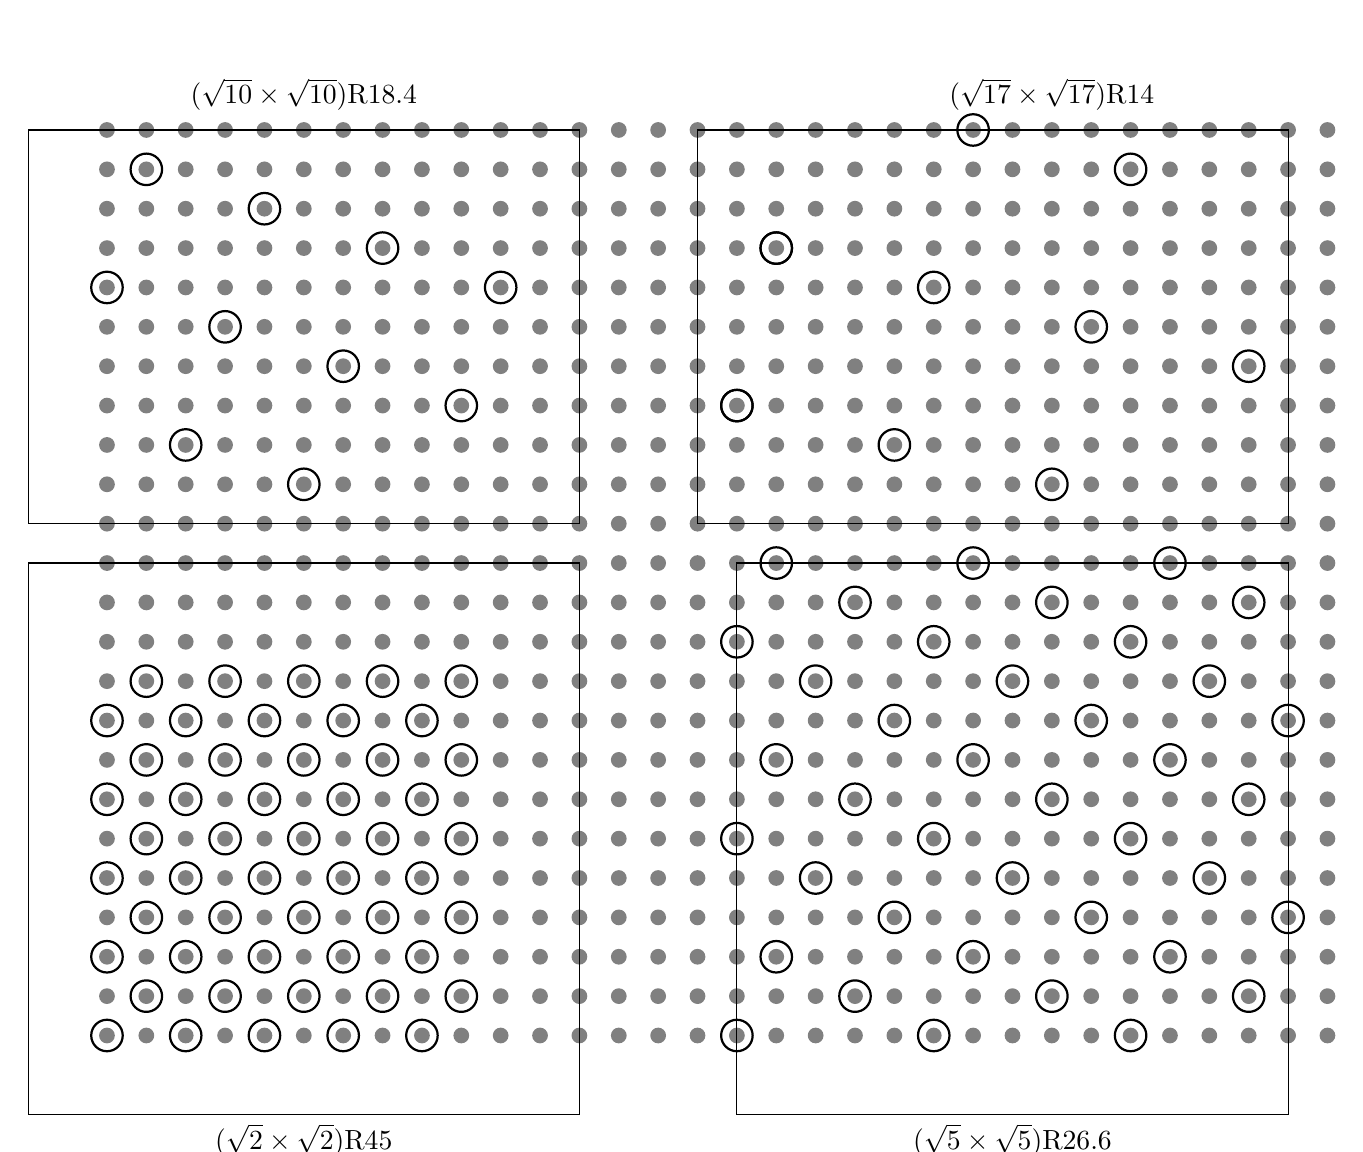
\begin{tikzpicture}
	\foreach \x in {0,0.5,1,...,15.5}
		\foreach \y in {0,0.5,1,...,11.5}
			{
			\fill[color=gray](\x,\y)circle (0.1cm);
			}
	
	%the 2x2R45
	\draw[-](-1,-1) --(6,-1) -- (6,6) --(-1,6)--cycle;
	\node at (2.5,-1)[anchor=north] {$(\sqrt{2}\times\sqrt{2})$R45};
	\foreach \x in {0,1,...,4}
		\foreach \y in {0,1,...,4}
			{
			\draw[thick](\x,\y) circle(0.2cm);
			}
	\foreach \x in {0.5,1.5,...,5}
		\foreach \y in {0.5,1.5,...,5}
			{
			\draw[thick] (\x,\y) circle (0.2cm);
			}
	
	%5x5R26.6
	\pgfmathsetmacro{\xshift}{8}
	\draw[-](8,-1)--(15,-1)--(15,6)--(8,6)--cycle;
	\foreach \x in {8,10.5,...,13}
		\foreach \y in {0,2.5,...,5}
			{
			\draw[thick] (\x,\y) circle (0.2cm);
			}
	\foreach \x in {9.5,12,...,14.5}
		\foreach \y in {0.5,3,...,5.5}
			{
			\draw[thick] (\x,\y) circle (0.2cm);
			}
	\foreach \x in {8.5,11,...,14.5}
		\foreach \y in {1,3.5,...,6}
			{
			\draw[thick] (\x,\y) circle (0.2cm);
			}
	\foreach \x in {10,12.5,...,15}
		\foreach \y in {1.5,4,...,4}
			{
			\draw[thick] (\x,\y) circle (0.2cm);
			}
	\foreach \x in {9,11.5,...,14}
		\foreach \y in {2,4.5,...,5.5}
			{
			\draw[thick] (\x,\y) circle (0.2cm);
			}
	\node at (11.5,-1)[anchor=north] {$(\sqrt{5}\times\sqrt{5})$R26.6};
	
	%10x10R18.4
	\draw[-](-1,6.5) -- (6,6.5) -- (6,11.5) -- (-1,11.5) -- cycle;
	\pgfmathsetmacro{\yshift}{7}
	\foreach \position in {(0,2.5+\yshift),(1,0.5+\yshift),(1.5,2+\yshift),(2.5,0+\yshift),(3,1.5+\yshift),(4.5,1+\yshift)}
		\draw[thick] \position circle (0.2cm);
	\foreach \position in {(0.5, 4+\yshift), (2,3.5+\yshift), (3.5, 3+\yshift),(5, 2.5+\yshift)}
		\draw[thick] \position circle (0.2cm);
	\node[label=above:$(\sqrt{10}\times\sqrt{10})$R18.4] at (2.5,11.5){};
	
	
	%17x17R14
	\draw[-](7.5,6.5) -- (15, 6.5) -- (15,11.5) -- (7.5,11.5) -- cycle;
	\foreach \position in {(0+\xshift,1+\yshift),(0.5+\xshift,3+\yshift)}
		\draw[thick] \position circle (0.2cm);
	\foreach \position in {(2+\xshift,0.5+\yshift),(2.5+\xshift,2.5+\yshift)}
		\draw[thick] \position circle (0.2cm);
	\foreach \position in {(4+\xshift,0+\yshift),(4.5+\xshift,2+\yshift)}
		\draw[thick] \position circle (0.2cm);
	\foreach \position in {(6.5+\xshift,1.5+\yshift)}
		\draw[thick] \position circle (0.2cm);
	\foreach \position in {(3+\xshift,4.5+\yshift),(5+\xshift,4+\yshift)}
		\draw[thick] \position circle (0.2cm);
	\foreach \position in {(0+\xshift,1+\yshift),(0.5+\xshift,3+\yshift)}
		\draw[thick] \position circle (0.2cm);
	\node[label=above:$(\sqrt{17}\times\sqrt{17})$R14] at (12,11.5){};
\end{tikzpicture}
\caption{Overlayer unit cells on substrate square lattice.}
\end{figure}


\subsection*{Part b}
The relative coverage is a simple division of areas.
\begin{align*}
	\text{Relative Coverage: } &\left(\sqrt{2}\times\sqrt{2}\right) \to 50\%\\[3mm]
		&\left(\sqrt{5}\times\sqrt{5}\right) \to 20\%\\[3mm]
		&\left(\sqrt{10}\times\sqrt{10}\right) \to 10\%\\[3mm]
		&\left(\sqrt{17}\times\sqrt{17}\right) \to 5.9\%\\[3mm]
\end{align*}


\subsection*{Part c}

\begin{figure}[H]
\centering
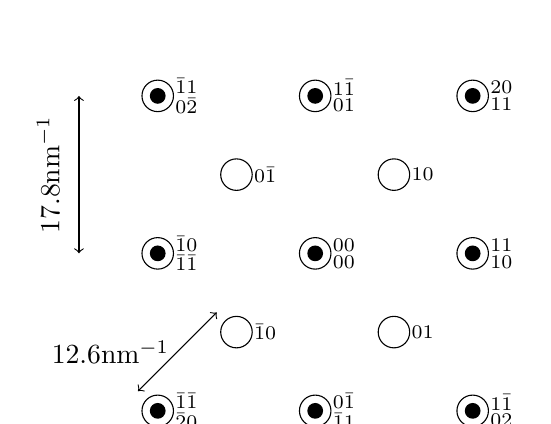
\begin{tikzpicture}
	\foreach \x in {0,2,4}
		\foreach \y in {0,2,4}
			{
			\fill(\x,\y)circle (0.1cm);
			\draw(\x,\y)circle (0.2cm);
			}
	\foreach \x in {1,3}
		\foreach \y in {1,3}
			\draw(\x,\y) circle(0.2cm);
			
	\draw[<->](-1,2) -- (-1,4);
	\node[label=left:\rotatebox{90}{$17.8$nm$^{-1}$}] at (-1,3){};
	
	\draw[<->](-0.25,0.25) -- (0.75,1.25);
	\node[label=center:$12.6$nm$^{-1}$] at (-0.6,0.75){};
	\node at (0.1,0)[anchor=west]{$_{\bar{2}0}^{\bar{1}\bar{1}}$};
	\node at (2.1,0)[anchor=west]{$_{\bar{1}1}^{0\bar{1}}$};
	\node at (4.1,0)[anchor=west]{$_{02}^{1\bar{1}}$};
	\node at (0.1,2)[anchor=west]{$_{\bar{1}\bar{1}}^{\bar{1}0}$};
	\node at (2.1,2)[anchor=west]{$_{00}^{00}$};
	\node at (4.1,2)[anchor=west]{$_{10}^{11}$};
	\node at (0.1,4)[anchor=west]{$_{0\bar{2}}^{\bar{1}1}$};
	\node at (2.1,4)[anchor=west]{$_{01}^{1\bar{1}}$};
	\node at (4.1,4)[anchor=west]{$_{11}^{20}$};
	\node at (1.1,1)[anchor=west]{$_{\bar{1}0}$};
	\node at (3.1,1)[anchor=west]{$_{01}$};
	\node at (1.1,3)[anchor=west]{$_{0\bar{1}}$};
	\node at (3.1,3)[anchor=west]{$_{10}$};
\end{tikzpicture}
\caption{LEED pattern. The filled circles and supercript correspond to Ni, while the open circles and the subscript corresponds to the O.}
\label{leed}
\end{figure}

We want to calculate the polar and azimuthal angles of the 13 innermost LEED spots. We first find the momentum of the electron beam with $E=150$ eV.
\begin{align*}
	\lambda &= \dfrac{h}{\sqrt{2mE}}\\[3mm]
		&= \dfrac{6.626\times 10^{-34}\,\,\text{J$\cdot$s}}{\left(2.9\times10^{11}\,\,\text{kg}\cdot 150\,\,\text{eV}\cdot 1.609\times10^{-19}\,\,\text{J/eV}\right)^{1/2}}\\[3mm]
		&= 0.1\,\,\text{nm}
\end{align*}
With this we can find the momentum,
\begin{align*}
|k| &= \dfrac{2\pi}{\lambda}\\[3mm]
	&= 62.8 \,\, \text{nm}^{-1}
\end{align*}

Next we find the length of the reciprocal lattice vectors. Ni is an FCC lattice with $a_0 = \SI{3.52}{\angstrom} = 0.352$nm.
\begin{align*}
|g_0| &= \dfrac{2\pi}{0.352}\\[3mm]
	&= 17.8\,\,\text{nm}^{-1}
\end{align*}
The surface lattice spacing is just scaling of the Ni FCC lattice with $a_0 = a_0(Ni)\cdot \sqrt{2} = 0.498$nm.
\[
|g_0| = 12.6\,\,\text{nm}^{-1}
\]

Now consider a section of the ewald sphere shown in figure \ref{ewald}. With some simple triginometry we can find the polar angle ($\phi$).
\[
	\phi = \arcsin\left(\dfrac{|g|}{|k_e|}\right)
\]
\begin{figure}[H]
\centering
\tdplotsetmaincoords{60}{110}
%
\pgfmathsetmacro{\rvec}{1}
\pgfmathsetmacro{\thetavec}{30}
\pgfmathsetmacro{\phivec}{60}
%
\begin{tikzpicture}[scale=5,tdplot_main_coords]
\coordinate (O) at (0,0,0);
\draw[thick,-] (0,0,0) -- (1,0,0);
\draw[thick,-] (0,0,0) -- (0,1,0);
\draw[thick,-] (0,0,0) -- (0,0,1);
\tdplotsetcoord{P}{\rvec}{\thetavec}{\phivec}
\draw[-stealth,color=red] (O) -- (P);
\draw[dashed, color=red] (O) -- (Pxy);
\draw[dashed, color=red] (P) -- (Pxy);
\tdplotdrawarc{(O)}{0.2}{0}{\phivec}{anchor=north}{$\theta$}
\tdplotsetthetaplanecoords{\phivec}
\tdplotdrawarc[tdplot_rotated_coords]{(0,0,0)}{0.5}{0}%
{\thetavec}{anchor=south west}{$\phi$}
\draw[dashed,tdplot_rotated_coords] (\rvec,0,0) arc (0:90:\rvec);
\draw[dashed] (\rvec,0,0) arc (0:90:\rvec);
\tdplotsetrotatedcoords{\phivec}{\thetavec}{0}
\tdplotsetrotatedcoordsorigin{(P)}
\end{tikzpicture}
\caption{Section of the ewald sphere.}
\label{ewald}
\end{figure}

Running all the calculations we get,
\begin{center}
 \begin{tabular}{||c c c c c||} 
 \hline
 Ni & O & $\vert$ g $\vert$ (nm$^{-1}$) & $\theta$ ($^\circ$) & $\phi$ ($^\circ$)\\ [0.5ex] 
 \hline\hline
 00 & 00 & 0 & 0 & 0 \\[1ex] 
 - & 10 & 12.6 & 45 & 11.6 \\[1ex] 
 - & 01 & 12.6 & 135 & 11.6 \\[1ex] 
 - & $\bar{1}$0 & 12.6 & 225 & 11.6 \\[1ex] 
 - & 0$\bar{1}$ & 12.6 & 315 & 11.6 \\[1ex] 
 10 & 11 & 17.8 & 90 & 16.5 \\[1ex] 
 $\bar{1}0$ & $\bar{1}\bar{1}$ & 17.8 & 270 & 16.5 \\[1ex] 
 01 & 1$\bar{1}$ & 17.8 & 0 & 16.5 \\[1ex] 
 0$\bar{1}$ & $\bar{1}$1 & 17.8 & 180 & 16.5 \\[1ex] 
 11 & 20 & 25.2 & 45 & 23.7 \\[1ex] 
 $\bar{1}$1 & 0$\bar{2}$ & 25.2 & 315 & 23.7 \\[1ex] 
 1$\bar{1}$ & 02 & 252 & 135 & 23.7 \\[1ex] 
 $\bar{1}\bar{1}$ & $\bar{2}$0 & 25.2 & 225 & 23.7 \\[1ex] 
 $\bar{1}\bar{1}$ & $\bar{2}0$ & 25.2 & 225 & 23.7 \\ [2ex] 
 \hline
\end{tabular}
\end{center}
%%%%%%%%%%%%%%%%%%%%%%%%%%%%%%%%%%%%%%%%%%%%%%%%%%%%%%%%%%%%%%%%%%%%%%%%%%%%%%%%%%%
%%%%%%%%%%%%%%% PROBLEM 8 %%%%%%%%%%%%%%%%%%%%%
%%%%%%%%%%%%%%%%%%%%%%%%%%%%%%%%%%%%%%%%%%%%%%%%%%%%%%%%%%%%%%%%%%%%%%%%%%%%%%%%%%%


\newpage
\section*{1.8}
\begin{bclogo}[logo=\bcquestion , barre=none]
\newline
For background, see Zangwill pp. 49-52, and more detailed discussion in excerpts from Desjonqueres and Spanjaard downloadable from course website, pages 571-578.
The current in an STM experiment can be approximately calculated from the simple proportionality relation
\[
	I \propto e^{-2\kappa L},
\]
with L the distance between tip and surface and $\kappa$ the usual quantity in barrier tunneling problems. The potential barrier inside $\kappa$ can be taken to be the work function of the surface, and we will take it to be 4.0 eV.
\vspace{2mm}
\newline
If the tip is brought to within 5 Å of the surface, with what precision in \% would the tunneling current have to be measured to reliably detect a change in surface height of 0.1 Å? Note that the precision will have to be about 10x better than the effect you want to see to be able to measure it accurately.
\end{bclogo}
\vspace{2cm}


\begin{align*}
	\dfrac{I(\SI{5.1}{\angstrom})}{I(\SI{5.0}{\angstrom})} &= \dfrac{e^{-2\kappa \SI{5.1}{\angstrom}}}{e^{-2\kappa \SI{5.0}{\angstrom}}}
		= 1.105\\[4mm]
	\dfrac{I(\SI{4.9}{\angstrom})}{I(\SI{5.0}{\angstrom})} &= \dfrac{e^{-2\kappa \SI{4.9}{\angstrom}}}{e^{-2\kappa \SI{5.0}{\angstrom}}}
		= 0.905
\end{align*}

Changing the tip-to-surface distance by $\SI{0.1}{\angstrom}$ causes a current change of approximately 10\%. We need a precision that is 10x better than this effect to be able to measure accurately. Thus the tunneling current must be precise to 1\% in order to relably detect a change in surface height of $\SI{0.1}{\angstrom}$.











\end{document}
